\documentclass{article}
\usepackage[margin=1in]{geometry}
\usepackage{booktabs}
\usepackage{graphicx}
\usepackage{hyperref}
\usepackage{amsmath}

\title{Diffusion: Regionally-Adaptive Cyclic Diffusion}
\author{Ansh}
\date{SAiDL Summer Assignment 2026}

\begin{document}
\maketitle

\section{Overview}

This report studies Regionally-Adaptive Cyclic Diffusion (RACD) for
unconditional landscape image generation. The system is implemented as latent
diffusion: images are resized to $256 \times 256$, encoded with a frozen
pretrained VAE, generated in the $32 \times 32$ latent space, and decoded only
for visualization and evaluation.

The assignment asks for three generation settings: a baseline DiT, a global
cyclic refinement baseline, and RACD. The primary question is whether adaptive
spatial refinement can approach the fidelity of global cyclic refinement while
spending less generation time.

\section{Assignment Compliance}

\begin{table}[h]
\centering
\begin{tabular}{ll}
\toprule
Requirement & Implementation \\
\midrule
Landscape dataset, no class conditioning & Kaggle \texttt{arnaud58/landscape-pictures}, unconditional model \\
Images resized to $256 \times 256$ & Dataset transform resizes/crops to $256 \times 256$ \\
Latent diffusion only & Frozen SD VAE, no pixel-space diffusion training \\
Fixed DiT baseline & Final run uses a fixed DiT-S/4 latent model \\
Global cyclic refinement & Noise to $t=200$, DDIM denoise back to $t=0$ \\
Difficulty predictor & Frozen DiT features to $32 \times 32$ difficulty map \\
RACD thresholding & Refine where $M > \tau$ \\
FID, CMMD, time & Evaluation scripts and sampling summaries provided \\
CMMD vs. compute tau sweep & Automated by \texttt{diffusion/run\_tau\_sweep.py} \\
Generated images in report & Grid generated by \texttt{diffusion/make\_sample\_grid.py} \\
\bottomrule
\end{tabular}
\caption{Mapping from the PDF diffusion requirements to the implementation.}
\end{table}

\section{Method}

\subsection{Baseline Latent DiT}

The final reported baseline is a fixed DiT-S/4-style transformer over VAE
latents. The model uses 4 input latent channels, a $32 \times 32$ latent grid,
patch size 4, hidden size 384, 6 transformer blocks, 6 attention heads, and
AdaLN-Zero timestep conditioning. I initially trained a DiT-B/8-style model,
but its $4 \times 4$ token grid became a visible spatial bottleneck under the
available Kaggle compute. The final DiT-S/4 configuration uses a smaller
transformer but a denser $8 \times 8$ token grid, which gave substantially
more coherent landscape structure. The model predicts the diffusion noise
$\epsilon$ and is trained with mean squared error:
\[
  \mathcal{L}_{\mathrm{DiT}} =
  \mathbb{E}_{z_0, t, \epsilon}
  \left[
    \left\| \epsilon_\theta(z_t, t) - \epsilon \right\|_2^2
  \right].
\]

Training uses AdamW with weight decay, gradient clipping, EMA weights, mixed
precision, linear warmup, and cosine learning-rate decay. The final checkpoint
was trained for 100k optimizer steps.

\subsection{Training Diagnostics and Checkpoint Selection}

During training, I initially monitored generated grids using the EMA copy of
the DiT. In the early B/8 run, this produced highly noisy samples even after
thousands of optimizer steps. Rather than treating this as conclusive model
failure, I compared EMA sampling against the raw checkpoint weights. At step
16000, the raw weights already produced recognizable landscape structure, while
the EMA samples were still dominated by high-frequency color noise.

The diagnosis was that an EMA decay of 0.9999 was too slow to use as the only
visual monitor in a short Kaggle-scale run. For the final S/4 run I used a
lower EMA decay of 0.999 and compared raw-vs-EMA samples during training; by
32k--50k steps the two were visually aligned, so the final evaluation uses EMA
weights. This debugging step also changed the training workflow: checkpoints
and sample grids are uploaded as W\&B artifacts so interrupted Kaggle sessions
can be resumed instead of restarting from scratch.

\subsection{Global Cyclic Refinement}

After standard DDIM sampling reaches $z_0$, global cyclic refinement applies
forward noise to timestep $t=200$ and denoises back to $t=0$. The refinement
uses the same DDIM update rule as the baseline sampler, which keeps the timing
comparison between baseline, global cyclic, and RACD meaningful.

\subsection{Difficulty Predictor}

The DiT is frozen before training the difficulty predictor. For each training
image, a latent $z_0$ is noised to a fixed intermediate timestep $t_{\mathrm{mid}}$.
The frozen DiT predicts noise, which is converted into
\[
  \hat{z}_0 =
  \frac{z_t - \sqrt{1-\bar{\alpha}_t}\epsilon_\theta(z_t,t)}
       {\sqrt{\bar{\alpha}_t}}.
\]
The target difficulty map is the normalized per-location squared error between
$\hat{z}_0$ and the clean latent $z_0$. A lightweight convolutional predictor
maps intermediate DiT token features to $M \in [0,1]^{32 \times 32}$.

The same feature timestep used to generate supervision is forced into the DDIM
sampling schedule at inference, preventing a train/test feature mismatch.

\subsection{RACD Masked Refinement}

At sampling time, RACD thresholds the difficulty map:
\[
  m_{ij} = \mathbf{1}[M_{ij} > \tau].
\]
The masked refinement implementation uses timestep-consistent blending. At
each denoising step, the unmasked region is re-injected from the known forward
process at the current timestep, while the masked region follows the denoising
trajectory. This avoids feeding the DiT a spatial mixture of $t=0$ and
$t=200$ latents in the same forward pass.

\section{Evaluation Protocol}

For each method, the sampler records average generation time per image. The
generated folders are compared against held-out real validation images using
FID and CMMD. CMMD is computed with CLIP image embeddings and an RBF-kernel MMD,
which avoids the Gaussian feature assumption used by FID.

The threshold sweep uses
\[
  \tau \in \{0.1, 0.2, 0.3, 0.4, 0.5, 0.6, 0.7, 0.8, 0.9\}.
\]
The selected threshold is the RACD point that minimizes the sum of normalized
CMMD and normalized generation time. This rule makes the fidelity/compute
trade-off explicit; the final discussion should also inspect the plotted
Pareto frontier rather than relying only on the scalar score.

\section{Results}

\begin{table}[h]
\centering
\begin{tabular}{lrrrr}
\toprule
Method & FID $\downarrow$ & CMMD $\downarrow$ & Time (s/img) & Refined Fraction \\
\midrule
Baseline DiT-S/4 & 184.55 & 0.0010093 & 0.1546 & 0.00 \\
Global Cyclic & 183.32 & 0.0009822 & 0.1953 & 1.00 \\
RACD $\tau=0.2$ & 184.12 & 0.0009911 & 0.1997 & 0.0134 \\
\bottomrule
\end{tabular}
\caption{Main comparison from the 256-image S/4 sweep.}
\end{table}

\begin{table}[h]
\centering
\begin{tabular}{rrrr}
\toprule
$\tau$ & CMMD $\downarrow$ & Time (s/img) & Refined Fraction \\
\midrule
0.1 & 0.0009998 & 0.1993 & 0.684 \\
0.2 & 0.0009911 & 0.1997 & 0.013 \\
0.3 & 0.0010064 & 0.1932 & 0.0005 \\
0.4 & 0.0010202 & 0.1790 & 0.0001 \\
0.5 & 0.0010160 & 0.1664 & 0.000004 \\
0.6 & 0.0010095 & 0.1650 & 0.000 \\
0.7 & 0.0010095 & 0.1656 & 0.000 \\
0.8 & 0.0010095 & 0.1654 & 0.000 \\
0.9 & 0.0010095 & 0.1658 & 0.000 \\
\bottomrule
\end{tabular}
\caption{RACD threshold sweep.}
\end{table}

\IfFileExists{../results/diffusion/tau_sweep_s4/cmmd_vs_time.png}{
  \begin{figure}[h]
  \centering
  
\includegraphics[width=0.75\linewidth]{../results/diffusion/tau_sweep_s4/cmmd_vs_time.png}
  \caption{CMMD vs. generation time for the RACD threshold sweep.}
  \end{figure}
}{}

\IfFileExists{../results/diffusion/final_s4_sample_grid.png}{
  \begin{figure}[h]
  \centering
  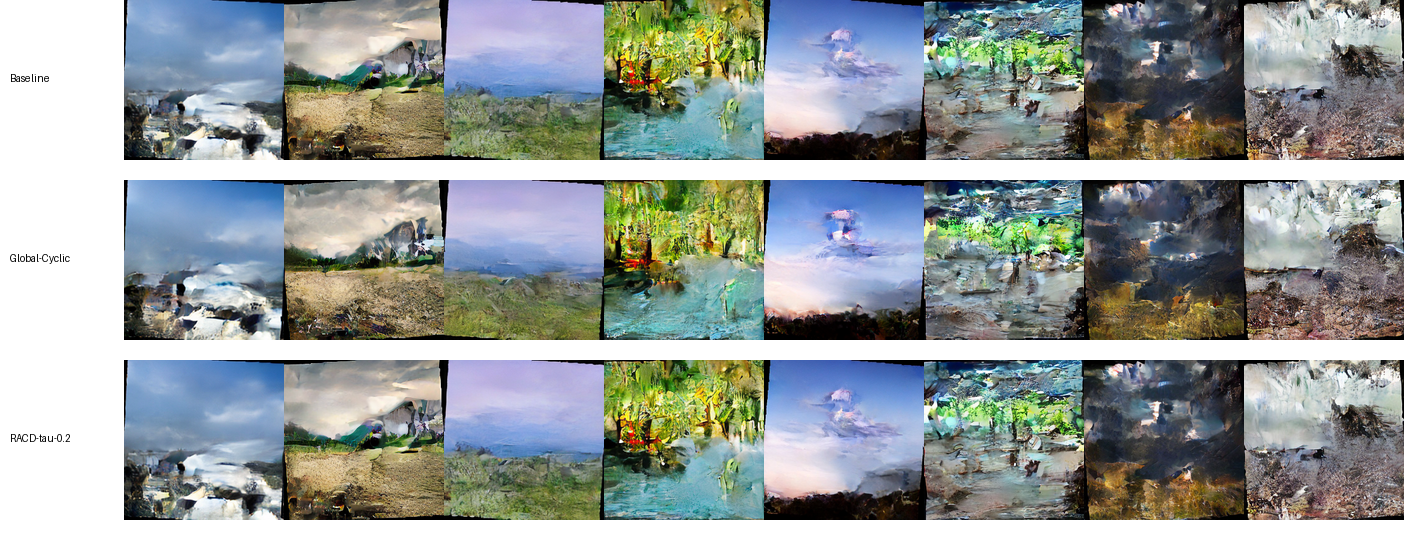
\includegraphics[width=\linewidth]{../results/diffusion/final_s4_sample_grid.png}
  \caption{Generated samples from baseline, global cyclic refinement, and RACD.}
  \end{figure}
}{}

\section{Analysis}

The final S/4 model is a substantial improvement over the earlier undertrained
B/8 checkpoint: FID dropped from the high 300s to 184.55, and CMMD dropped from
roughly $2.2 \times 10^{-3}$ to $1.0 \times 10^{-3}$. Visually, the samples now
show recognizable landscape composition, including sky, terrain, water-like
regions, and horizon structure, though they remain painterly rather than fully
photorealistic.

Global cyclic refinement produced the best FID and CMMD in this sweep. It
improved FID from 184.55 to 183.32 and CMMD from 0.0010093 to 0.0009822, with
generation time increasing from 0.1546 s/image to 0.1953 s/image. This confirms
that the cyclic denoising pass can improve sample fidelity, but at a measurable
compute cost.

The most meaningful RACD threshold was $\tau=0.2$: it improved over the
baseline CMMD while refining only 1.34\% of latent locations, and came close to
the global cyclic CMMD. Higher thresholds such as $\tau \ge 0.6$ became faster
after adding an empty-mask skip, but they selected no regions and therefore
collapsed to baseline behavior. The measured wall-clock time for the meaningful
RACD point is still close to global cyclic refinement because this
implementation performs the masked denoising pass as a dense latent operation.
Thus, the experiment validates the learned spatial difficulty map and
thresholding logic, while a more optimized patch-sparse implementation would be
needed to fully realize the intended wall-clock compute savings.

\section{Conclusion}

The implementation satisfies the main RACD pipeline required by the assignment:
baseline latent DiT sampling, global cyclic refinement, frozen-feature difficulty
prediction, masked RACD refinement, FID/CMMD/time measurement, and a tau sweep.
The final S/4 checkpoint produces recognizable landscape images and improves
substantially over the initial undertrained run. Global cyclic refinement gives
the strongest absolute metrics, while RACD demonstrates that the learned
difficulty predictor can identify a small set of regions whose refinement
nearly matches the global cyclic CMMD. The main remaining limitation is compute:
the current masked refinement is algorithmically region-aware but not yet
implemented with patch-sparse wall-clock savings.

\end{document}
